\documentclass[twoside,11pt]{article}

% Findings-first companion to ../main.tex (the system paper). Shares ../jmlr2e.sty,
% ../references.bib and ../figures. Build from inside paper/findings/:
%   pdflatex main && bibtex main && pdflatex main && pdflatex main
\usepackage[abbrvbib,preprint]{../jmlr2e}

\usepackage[T1]{fontenc}
\usepackage{lmodern}
\usepackage{microtype}
\usepackage{amsmath}
\usepackage{booktabs}
\usepackage{array}
\usepackage{tabularx}
\usepackage{xcolor}
\usepackage{enumitem}
\usepackage{tikz}
\usetikzlibrary{arrows.meta,positioning,fit,backgrounds,calc,decorations.pathreplacing}
\usepackage{lastpage}
\usepackage{caption}
\usepackage{subcaption}
\usepackage{pifont}
\usepackage{placeins}

\graphicspath{{../figures/}}
\setlist{itemsep=2pt,topsep=3pt}
\renewcommand{\topfraction}{0.9}
\renewcommand{\bottomfraction}{0.8}
\renewcommand{\textfraction}{0.07}
\renewcommand{\floatpagefraction}{0.85}
\setcounter{topnumber}{3}
\setcounter{totalnumber}{5}
\setlength{\emergencystretch}{3em}

\definecolor{tfm}{HTML}{2f6f8f}
\definecolor{ctwo}{HTML}{9b4f7f}
\definecolor{sun}{HTML}{3d7f5a}
\definecolor{bolt}{HTML}{8a6a3a}
\definecolor{timer}{HTML}{d08a2e}
\definecolor{tmoe}{HTML}{b5473f}
\definecolor{tt5}{HTML}{6a6fb0}
\definecolor{accent}{HTML}{c0602a}
\definecolor{soft}{HTML}{eef2f5}

\newcommand{\repourl}{https://github.com/DanK10097110/TSFM-Interp}
\newcommand{\repo}[1]{\href{\repourl/blob/main/#1}{\nolinkurl{#1}}}
\newcommand{\repodir}[1]{\href{\repourl/tree/main/#1}{\nolinkurl{#1}}}
\newcommand{\fid}[1]{\href{\repourl/blob/main/FINDINGS.md}{\textsf{#1}}}
\newcommand{\tool}{\textsc{TSFM-Lens}}
\newcommand{\cmark}{\ding{51}}
\newcommand{\xmark}{\ding{55}}
\newcommand{\ev}[1]{\textsc{#1}}

\jmlrheading{}{2026}{1-\pageref{LastPage}}{}{}{}{Daniel Kushnir and Hao Wang}
\ShortHeadings{What Time-Series Foundation Models Share}{Kushnir and Wang}
\firstpageno{1}

\begin{document}

\title{Same Inputs, Different Mechanisms:\\ What Seven Time-Series Foundation Models Share}

\author{\name Daniel Kushnir \email kushnir.daniel05@gmail.com \\
       \name Hao Wang (corresponding author) \email hoguewang@gmail.com \\
       \addr Rutgers University}

\editor{}

\maketitle

\begin{abstract}%
Time-series foundation models (TSFMs) differ sharply in architecture: decoder-only stacks over 32-step patches,
encoder--decoders over quantized single steps, encoders with cross-series attention, decoders with sampled heads. Do they
learn the same things? We compare seven TSFMs on a common, empirically measured time axis, with every causal instrument
validated on a forecaster with planted concepts and every registered claim tested once on a sealed held-out split, on
two independent corpora. Three conclusions emerge. \emph{First, the models agree on what in a series matters.} All 21
model pairs share representational geometry above a shuffled-series null on fresh data, and features in architecturally
unrelated models select the same series for a concept: all registered transfer claims confirm on both private splits
and on 800 raw real-world windows. \emph{Second, they implement the response differently.} Causal features
act mainly on forecast level and seasonality, and these broad effect types recur in all seven models, but fine-grained
concepts are organized by model (none spans more than three of seven), forecast-relevant information is spread over many
directions (single features exceed on-manifold random directions only 1.29-fold), and the same effect on the same series
is detected only within the Chronos family. \emph{Third, interpretability shortcuts imported from language models mislead
on TSFMs.} Averaging a window's tokens hides 0.30--0.43 of TimesFM's held-out similarity to fine-token models;
83.5\% of the most prominent dictionary features have no held-out causal effect; attention mass on seasonal lags does
not predict which heads carry seasonality; and a plausible null inflates the count of causal features 2.7-fold. Code,
benchmark and every result with its reproduction command are public.
\end{abstract}

\begin{keywords}
  time-series foundation models, mechanistic interpretability, representational similarity, sparse autoencoders,
  causal intervention
\end{keywords}

\section{Introduction}
\label{sec:intro}

Pretrained forecasting models such as TimesFM \citep{das2024timesfm}, the Chronos family
\citep{ansari2024chronos,ansari2025chronos2}, Sundial \citep{liu2025sundial}, Timer \citep{liu2024timer} and Time-MoE
\citep{shi2025timemoe} are released as open checkpoints and used zero-shot. They are built very differently. TimesFM
reads 32-step patches with a decoder; Chronos-T5 quantizes every time step into a vocabulary and runs an
encoder--decoder; Chronos-2 is an encoder with cross-series attention; Sundial samples its forecast from a flow-matching
head; Timer reads 96-step tokens. Benchmarks rank them by accuracy but do not tell us what they represent. In
vision and language, networks trained on similar data are argued to converge on similar representations
\citep{li2016convergent,huh2024platonic}. It is not known whether
forecasting models with such different inductive biases do the same, or whether any shared structure affects the
forecast.

We study this question for seven TSFMs. Three properties of forecasting models make the standard interpretability
toolkit \citep{kornblith2019cka,meng2022rome,bricken2023monosemanticity} hard to apply directly, and in each case the
failure is a plausible but wrong result rather than an error. Tokens cover between 1 and 96 time steps depending on the
model, so activations must be placed on a common time axis before they can be compared. Real series carry no labels for
trend, seasonality or noise, so a probe that appears to find seasonality cannot be checked on them. And removing a single
internal feature typically moves a forecast by about a tenth of the context's standard deviation, small enough that a
poorly chosen null or a precision mismatch can produce spurious effects. We therefore measure each model's token-to-time
map, use generated benchmarks with exact ground truth, validate the causal instruments on a forecaster with planted
concepts and decoys, and test registered claims once on sealed held-out splits of two corpora
(Section~\ref{sec:methods}).

Our results fall into three groups. The first concerns what the models share (Section~\ref{sec:shared}). All 21 model
pairs have representational geometry above chance, confirmed on a fresh sealed split, and concepts transfer across
architectures at the level of inputs. For a concept found in one model, features in the other models select the same
series, and all registered transfer claims confirm on both corpora and on 800 raw real-world windows that were never used
during development.

The second concerns how the models differ (Section~\ref{sec:mechanisms}). Causal features act mostly on the level and
seasonality of the forecast, and features that raise level, lower level or damp seasonality occur in every model.
Finer-grained concepts, however, are organized by model, and none spans more than three of the seven. The same function
can be implemented by one attention head in TimesFM and by five interacting heads in Chronos-T5-Base. Forecast-relevant
information also appears to be distributed, since single features stand out only modestly against random directions
drawn from the activation distribution. We detect the same causal effect on the same series only between Chronos-2 and
Chronos-Bolt.

The third concerns methodology (Section~\ref{sec:shortcuts}). Averaging the tokens in a time window, the usual way of
comparing models with different tokenizers, understates TimesFM's similarity to fine-token models by 0.30--0.43 CKA.
Of the most frequently and strongly active dictionary features, 83.5\% have no held-out causal effect. Attention to
seasonal lags is uncorrelated with which heads carry seasonality, and a random-direction null that ignores a feature's
per-token activation profile inflates the number of causal features 2.7-fold.

In addition, the depths at which TimesFM and Chronos-2 respond to input corruptions agree in a way that replicates for
most corruptions, and internal features improve failure prediction only for the two least accurate models
(Section~\ref{sec:depth}). Each result is recorded, with its evidence class, exact numbers and a reproduction command, in
a public findings ledger (\repo{FINDINGS.md}); identifiers such as \fid{SH-18} refer to its entries. The analysis
software and benchmark generator are open source (Appendix~\ref{app:system}).

\begin{figure}[!tb]
\centering
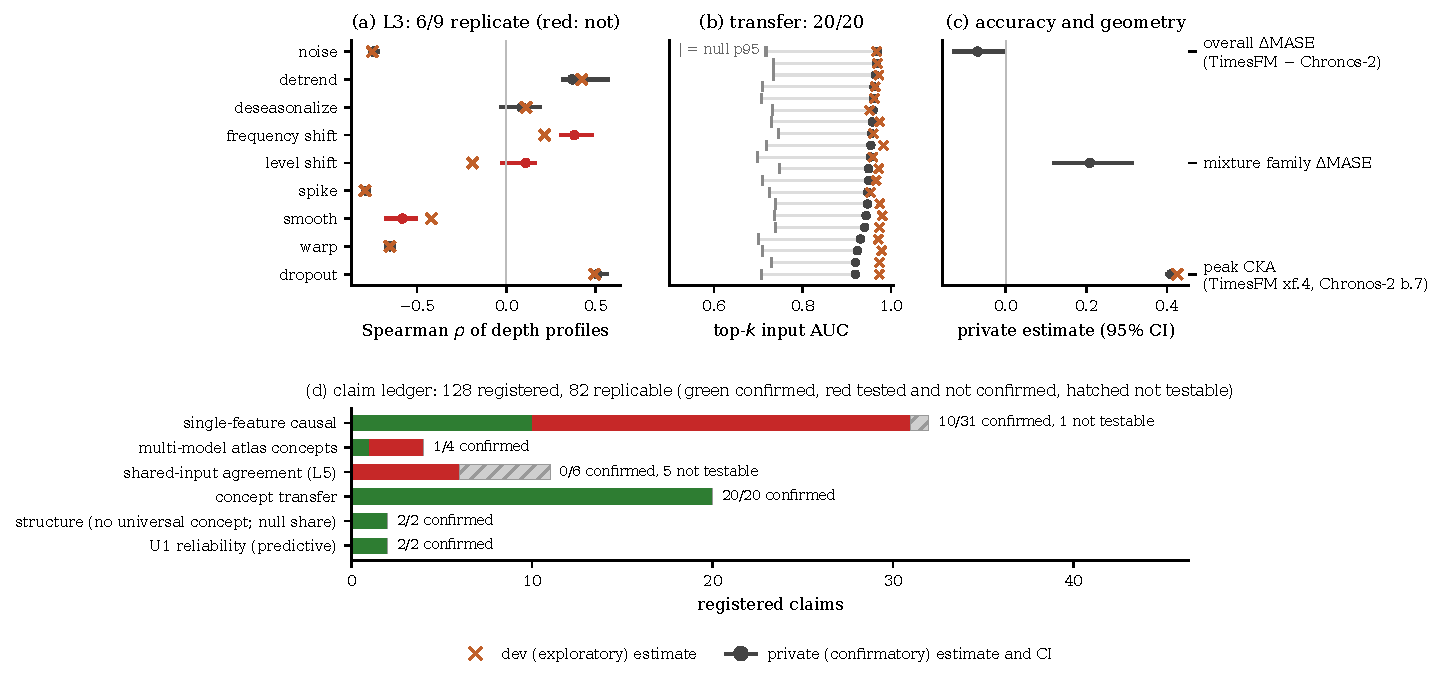
\includegraphics[width=\textwidth]{heldout.pdf}
\caption{Claims re-tested once on the sealed v2 private split (971 series; panel a uses 800 of them). (a) Per-corruption
depth-profile agreement, TimesFM vs.\ Chronos-2 (red: the dev value is not inside the private interval). (b) The 20
concept-transfer claims with private null 95th percentiles. (c) Accuracy and peak CKA; crosses are
dev values, dots and bars private values with 95\% series-bootstrap intervals. (d) Registered concept claims by
type. Source:
\texttt{confirm/confirmation.json}.}
\label{fig:heldout}
\end{figure}

\section{Related Work}
\label{sec:related}

\paragraph{Interpreting TSFMs.} \citet{wilinski2025exploring} study representational redundancy and concept steering in
TSFMs, and four recent studies train sparse autoencoders (SAEs) on a single TSFM
\citep{mishra2026dissecting,oublal2026timesae,divo2026zeitgeist,yildirim2026superposition}; \citet{kalnare2025mechts}
apply patching and SAEs to time-series classifiers, and saliency methods for time-series classifiers are unreliable
across architectures \citep{ismail2020benchmarking}. These works examine one model at a time and report features on
the data they were found on. We compare seven architectures on a common time axis, separate agreement on inputs from
agreement on effects, and test claims on held-out data. Our negative findings on activation prominence and on
single-feature specificity bear directly on the single-model SAE studies.

\paragraph{Comparing representations.} Representational similarity
\citep{raghu2017svcca,morcos2018pwcca,kornblith2019cka,kriegeskorte2008rsa} and model stitching
\citep{lenc2015equivariance,bansal2021stitching} underlie the convergence hypothesis for vision and language networks
\citep{li2016convergent,huh2024platonic}. We use them only against shuffled-series nulls and report stitching as a gain
over an input-feature baseline. Crosscoders \citep{lindsey2024crosscoders} learn one dictionary across models; we instead
compare independently trained dictionaries through the series they select and their effects on the forecast.

\paragraph{Validity of interpretability methods.} Probes need control tasks \citep{hewitt2019control,belinkov2022probing};
activation patching is sensitive to metric and corruption \citep{zhang2024patching,heimersheim2024patching}; subspace
interventions can create illusory mechanisms \citep{makelov2024illusion}; attention weights are not explanations
\citep{jain2019attention}; and SAE features vary across seeds \citep{paulo2025seeds}. Causal abstraction
\citep{geiger2021causal} formalizes when an intervention supports a mechanistic claim. We address these concerns
empirically with planted known answers, and borrow pre-registration \citep{nosek2018preregistration} and protection
against adaptive holdout reuse \citep{dwork2015reusable,gelman2014garden} from empirical science.

\section{Models and Data}
\label{sec:setup}

\paragraph{Models.} We analyze seven TSFMs (Table~\ref{tab:models}) spanning decoder-only, encoder-only and
encoder--decoder stacks, token widths from 1 to 96 steps, a mixture of experts, and deterministic and sampled heads.
Chronos-2 is the most accurate (median MASE 1.2002 on the v2 dev split, against 1.2560 for TimesFM and 1.9819 for the
seasonal-naive forecast), and on the private split it is more accurate than TimesFM on the registered \texttt{mixture}
family ($\Delta$MASE 0.209 [0.119, 0.313], $p_{\text{Holm}}=0.0002$, $n=290$; v3 0.303). Time-MoE is less accurate
than the naive forecast overall (median MASE 2.8642), so its internal results describe a model that does not forecast
these series well. Per-model behavior is summarized in Appendix~\ref{app:behavior}.

\begin{table}[!tb]
\centering
\footnotesize
\setlength{\tabcolsep}{4pt}
\resizebox{\textwidth}{!}{%
\begin{tabular}{@{}lllccrrr@{}}
\toprule
Model & Checkpoint & Architecture & Token & Head & Params & Median MASE & FLOPs obs. \\
\midrule
\textcolor{tfm}{TimesFM 2.5} & \texttt{google/timesfm-2.5-200m} & decoder-only & 32 & deterministic & 231M & 1.2560 & 42.5\% \\
\textcolor{ctwo}{Chronos-2} & \texttt{amazon/chronos-2} & encoder (+group attn.) & 16 & deterministic & 119M & 1.2002 & 97.5\% \\
\textcolor{sun}{Sundial} & \texttt{thuml/sundial-base-128m} & decoder + flow head & 16 & sampled & 128M & 1.4131 & 21.3\% \\
\textcolor{bolt}{Chronos-Bolt} & \texttt{amazon/chronos-bolt-small} & encoder + patch head & 16 & deterministic & 48M & 1.5487 & 79.1\% \\
\textcolor{tt5}{Chronos-T5-Base} & \texttt{amazon/chronos-t5-base} & encoder--decoder & 1 & sampled & 201M & 1.4231 & 13.9\%$^{a}$ \\
\textcolor{timer}{Timer} & \texttt{thuml/timer-base-84m} & decoder-only & 96 & deterministic & 84M & 1.9306 & 99.8\% \\
\textcolor{tmoe}{Time-MoE} & \texttt{Maple728/TimeMoE-50M} & decoder-only, MoE & 1 & deterministic & 113M & 2.8642 & 50.0\% \\
\bottomrule
\end{tabular}}
\caption{The seven models. ``Token'' is time steps per token; median MASE is on the v2 dev split (965 series;
seasonal naive 1.9819); ``FLOPs obs.''\ is the share of a forecast's FLOPs spent in captured blocks at context 480.
$^{a}$Encoder only; the sampled decoder is not captured (\fid{DE-05}).}
\label{tab:models}
\end{table}

\paragraph{Benchmarks with ground truth.} Real series offer no ground truth for concepts, so every analysis runs on
generated corpora in two labeled tiers. The \emph{synthetic} tier touches no real data and records every generative
component (trend, multiple seasonalities, AR noise, changepoints, anomalies, random walk, intermittency,
heteroskedasticity). The \emph{real-derived} tier (mixtures, block bootstrap \citep{kunsch1989block}, sequential
synthesis) inherits real source distributions and has attributional ground truth only. Every sample passes a leakage gate
against the Monash archive \citep{godahewa2021monash} by banded DTW \citep{sakoe1978dtw}. Each corpus has a dev split for
exploration and a sealed private split from a disjoint seed range, hashed so that any change is detected.
\begin{itemize}
  \item \textbf{v2} (primary): 965 dev series in five generator families, 410 of them real-derived (Monash weather, ETT
    \citep{zhou2021informer}, electricity and traffic), and 971 private series.
  \item \textbf{v3} (replication): 2{,}876 dev series, 785 real-derived from 15 sources, and 1{,}024 private series. An
    \emph{external} set of 800 raw windows from 12 GIFT-Eval datasets \citep{aksu2024gifteval}, cut without any
    generator, re-tests the registered transfer claims, and a second sealed epoch tests the registered geometry claims.
\end{itemize}
Dev and private splits are exchangeable on both corpora (energy-distance $p=0.951$ and $0.995$; \fid{MP-09}). Contexts
have 480 steps and the horizon 64 steps.

\paragraph{Explore, then confirm once.} Everything measured on a dev split is exploratory. Selected dev results are
frozen as hypotheses in a hash-pinned registry (v2: 128 hypotheses, 82 replicable on the private split; v3: 111 and 63)
before the private split is generated, and each is tested once. Every interval and $p$-value resamples whole series,
never windows \citep{efron1993bootstrap,cameron2008cluster}; each claim type is a Holm family \citep{holm1979}. On v2, 43
of 82 replicable claims confirm; on v3, 41 of 63 (Table~\ref{tab:heldout}). The pattern is identical on both corpora and
organizes the rest of the paper: claims about geometry and shared inputs replicate, single-feature causal claims
replicate in part, and claims that two models share a causal effect do not.

\begin{table}[!tb]
\centering
\footnotesize
\begin{tabular}{@{}lccc@{}}
\toprule
Registered claim type & v2 (971 series) & v3 (1{,}024 series) & Section \\
\midrule
Accuracy (Chronos-2 better on \texttt{mixture}) & 1/1 & 1/1 & \ref{sec:setup} \\
Peak-CKA pair & 1/1 & 1/1 & \ref{sec:geometry} \\
Concept transfer (shared inputs) & 20/20 & 20/20 & \ref{sec:inputs} \\
\quad same claims on 800 raw real windows & -- & 20/20 & \ref{sec:inputs} \\
Atlas structure & 2/2 & 2/2 & \ref{sec:bymodel} \\
Single-model atlas concept & 1/1 & -- & \ref{sec:bymodel} \\
Cross-model causal (atlas concepts; agreement) & 0/3; 0/6 & none registrable & \ref{sec:sameeffect} \\
Single-feature causal effect & 10/31 & 11/24 & \ref{sec:distributed} \\
Perturbation-profile agreement & 6/9 & 4/9 & \ref{sec:depth} \\
Failure prediction from internals & 2/2 & 2/3 & \ref{sec:depth} \\
\midrule
Confirmed / replicable (not testable) & 43/82 (6) & 41/63 (3) & \\
\midrule
Window geometry, second sealed v3 split: & & & \\
\quad 21 pairs above null; mean understates 4 pairs & -- & 21/21; 4/4 & \ref{sec:geometry} \\
\bottomrule
\end{tabular}
\caption{Held-out confirmation on two independent corpora. Each cell is confirmed / tested; each claim type is one Holm
family. The external raw-window set and the second v3 split (512 of its 2{,}863 series used) are not counted in the
totals (\fid{CA-11}, \fid{CA-12}).}
\label{tab:heldout}
\end{table}

\section{How Models Are Compared}
\label{sec:methods}

\subsection{A common time axis}
\label{sec:alignment}

A 480-step context is 480 tokens in Chronos-T5 and Time-MoE, 30 in Chronos-2, Sundial and Chronos-Bolt, 15 in TimesFM
and 5 in Timer, so token positions cannot be compared across models. We measure each token's time span $I_j$ by
injecting an impulse at every time step and accepting a span only if it passes contrast and contiguity gates (spans of
all six hand-written adapters are recovered exactly from measurement; \fid{MP-01}). Every model's tokens are then placed
on one grid of windows $W_w=[wL,(w+1)L)$, $L=32$ steps (Figure~\ref{fig:alignment}), and a window is represented by its
tokens concatenated in time order,
\begin{equation}
  \tilde h_w = \big[\,h_j\,\big]_{I_j\subseteq W_w}.
  \label{eq:pooling}
\end{equation}
A token as long as a window maps to it one to one, and Timer's 96-step token is copied to the three windows it spans.
Concatenation loses nothing, and linear CKA needs only the Gram matrix $K=\sum_p X_pX_p^{\top}$ summed over token
positions, so the long vector is never formed. Alignment fixes the \emph{rows} of two models' activations, not their
coordinates, so every cross-model measure is defined on shared rows: geometry compares how rows relate within each model,
concept transfer compares which series a feature selects, and causal effects are compared on the forecast. Activations
are never moved between models. During extraction an alignment gate checks, layer by layer, that an impulse in a window
is answered most strongly by that window.

\begin{figure}[!tb]
\centering
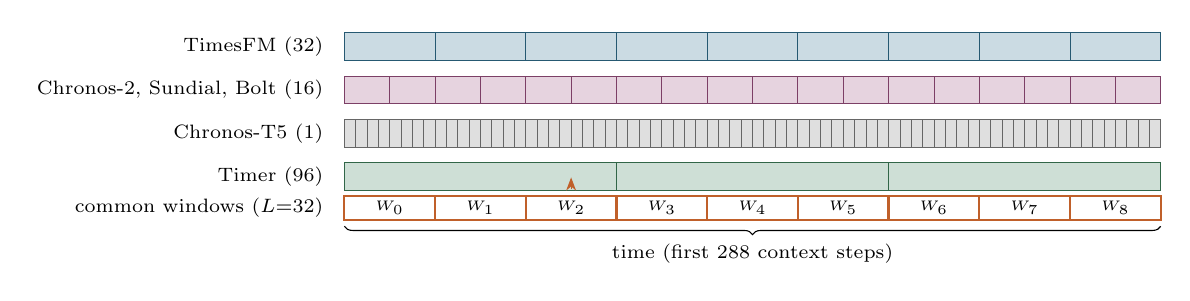
\begin{tikzpicture}[x=0.36mm,y=5.5mm,font=\scriptsize]
  \foreach \row/\name/\w/\col in {3/TimesFM (32)/32/tfm, 2/{Chronos-2, Sundial, Bolt (16)}/16/ctwo, 1/Chronos-T5 (1)/4/gray, 0/Timer (96)/96/sun}{
    \node[anchor=east] at (-4,\row) {\name};
    \pgfmathtruncatemacro{\n}{288/\w-1}
    \foreach \k in {0,...,\n}{
      \draw[fill=\col!25, draw=\col!80!black, line width=0.3pt] (\k*\w,\row-0.32) rectangle ({(\k+1)*\w},\row+0.32);
    }
  }
  \foreach \k in {0,...,8}{
    \draw[thick, accent] (\k*32,-1.0) rectangle ({(\k+1)*32},-0.45);
    \node[font=\tiny] at (\k*32+16,-0.72) {$W_{\k}$};
  }
  \node[anchor=east] at (-4,-0.72) {common windows ($L{=}32$)};
  \draw[-{Stealth}, accent] (80,-0.3) -- (80,-0.02);
  \draw[decorate,decoration={brace,amplitude=3pt,mirror}] (0,-1.15) -- (288,-1.15) node[midway,below=3pt] {time (first 288 context steps)};
\end{tikzpicture}
\caption{Time alignment. Tokens cover measured spans of different widths (Chronos-T5's one-step tokens are drawn in
groups of four). Equation~\eqref{eq:pooling} places them on common 32-step windows: shorter tokens are concatenated in
time order, TimesFM's tokens map one to one, and each Timer token is copied to the three windows it spans.}
\label{fig:alignment}
\end{figure}

\subsection{Geometry}

For aligned, centered window representations $A$ and $B$ over the same series, linear CKA \citep{kornblith2019cka},
$\mathrm{CKA}(A,B)=\|B^{\top}A\|_F^2/(\|A^{\top}A\|_F\|B^{\top}B\|_F)$, is computed for every layer pair of every model
pair and read against a null that permutes whole series (1{,}000 permutations). Ridge stitching
\citep{bansal2021stitching} is reported only as its gain over a map from input features, since much of any layer is
linearly predictable from the input alone.

\subsection{Causal features}
\label{sec:causal}

\paragraph{Dictionaries and ablation.} Each target layer $\ell$ receives a TopK sparse autoencoder
\citep{makhzani2013ksparse,gao2025topk}, $z(h)=\operatorname{TopK}(W_e(h-b_d)+b_e)$, $\hat h=W_dz(h)+b_d$, with three
replicate seeds. Feature $i$ is tested on the $k$ series on which it fires most strongly by comparing the forecast under
the reconstruction with $z_i=0$, $\hat h_{-i}$, against the forecast under the full reconstruction,
\begin{equation}
  \Delta_i^{(c)}(x) = g_c\big(f(x;h^{(\ell)}\!\leftarrow\!\hat h_{-i})\big) - g_c\big(f(x;h^{(\ell)}\!\leftarrow\!\hat h)\big),
  \label{eq:ablation}
\end{equation}
on nine forecast \emph{channels} $g_c$: trend, seasonal strength, spectral centroid, level, dispersion, near- and
far-horizon shape distance, MASE and flatness. Using the reconstruction in both arms keeps the dictionary's own error
out of the comparison. Before any feature is scored, a reach probe requires that patching a layer into itself changes
the forecast by exactly 0.0 and that patching another layer changes it, and sampled models are seeded identically in
compared calls.

\paragraph{Random-direction nulls.} A feature counts as causal on channel $c$ only if its mean $|\Delta_i^{(c)}|$ exceeds
the 95th percentile of removing the \emph{same amount} of activation, token by token, along 16 random directions on the
same series. Two direction distributions are used. The \emph{isotropic} null (v2) draws directions uniformly in the
dictionary's code space and decodes them. The \emph{covariance-matched} null (v3) draws them from a Gaussian with the
layer's own activation covariance, so they lie in the subspace the model actually uses. A feature's effect vector
$v_i^{(c)}$ is its signed mean effect in units of its null's 95th percentile. Because a mean is compared with a
percentile of single rows, the chance rate of clearing is estimated per cell by scoring each null draw against the
others.

\paragraph{From features to concepts.} Within a layer, causal features are clustered by effect vector ($k$-means,
silhouette, at least three members per cluster). Across models, the \emph{atlas} pools all causal features and cuts a
complete-linkage dendrogram at cosine 0.9, so an atlas concept is a tight causal-effect profile; coarser \emph{families}
(average linkage at cosine 0.5) serve as a reading vocabulary.

\subsection{Two kinds of sharing}
\label{sec:sharing}

Whether a concept is shared between two models is two questions. \emph{Same inputs}: concept transfer asks whether some
feature in another model separates a concept's top-$k$ series from the rest (AUC), against stratum-matched random series
sets; it is run in both directions with Benjamini--Hochberg control \citep{benjamini1995fdr}. \emph{Same effect on the
same inputs}: for every reciprocal transfer, both sides are ablated on the same series; each must clear its own null,
and their level concordance and shape cosine must exceed floors obtained by ablating random feature sets matched to each
side's activation. A statistic below both floors' 5th percentile means the two \emph{act differently}; merely failing
to exceed the 95th percentile is not evidence of a difference.

\subsection{Validation on known answers}
\label{sec:knownanswer}

A null can be wrong without raising any error, so each instrument is first run on a forecaster with planted concepts.
One block of this forecaster writes known directions into the residual stream on series with a given property, and the
head applies a known effect on level, trend, seasonality or dispersion. Decoys include input-only directions with no
effect, sub-null directions with a weak effect and a control layer with none; for cross-model tests, two architectures
with rotated residual bases share planted concepts. Pass criteria were fixed in advance and evaluated on five
construction seeds (Table~\ref{tab:knownanswer}). Both nulls used in the study pass. The test can fail a method: a
plausible null that removes one batch-averaged amount instead of each token's own profile fails on every seed and, on a
four-model development run, inflates the number of causal features from 110 to 293 (\fid{MN-29}). The
same-effect test never calls a decoy ``same'' but rarely detects a concept two architectures truly share
(\fid{MN-30}), so its positive verdicts are trustworthy and its silence is uninformative.

\begin{table}[!tb]
\centering
\footnotesize
\setlength{\tabcolsep}{4pt}
\begin{tabularx}{\textwidth}{@{}>{\raggedright}p{4.4cm}>{\raggedright}X>{\raggedright}p{3.0cm}c@{}}
\toprule
Instrument & Result on the planted forecaster & Pass criterion & Verdict \\
\midrule
Isotropic null (v2) & false-positive rate $\le$0.003, sensitivity 0.70--1.00, all 5 seeds & FPR $\le$0.10, sens.\ $\ge$0.5 & pass \\
Covariance-matched null (v3) & sensitivity 0.916, false positives in 5 of 2{,}948 control cells & FPR $\le$0.10, sens.\ $\ge$0.5 & pass \\
Batch-averaged null (reference) & false-positive rate 0.168--0.248 on every seed & FPR $\le$0.10, sens.\ $\ge$0.5 & fail \\
Same effect on same inputs & false ``same'' 0 of 9 decoys; detects a shared one-direction concept in 0.4 of seeds & -- & specific, insensitive \\
\bottomrule
\end{tabularx}
\caption{Known-answer tests of the causal instruments, with criteria fixed before each test (\fid{MN-29},
\fid{MN-30}).}
\label{tab:knownanswer}
\end{table}

\section{Shared Structure Across Architectures}
\label{sec:shared}

\subsection{Representational geometry}
\label{sec:geometry}

With concatenated windows, peak CKA (the maximum over layer pairs) between TimesFM and each other model is 0.358--0.635
on v2 and 0.375--0.712 on v3 (512 series each), and all 21 model pairs exceed their shuffled-series null on both corpora
($p=0.001$, 1{,}000 permutations; null 95th percentiles 0.003--0.51, highest for pairs with Time-MoE). The layer pairs
selected on v3 dev were registered and tested once on a fresh sealed split, and all 21 exceed their nulls (Holm $p=0.021$),
with TimesFM/Chronos-2 at 0.707 [0.679, 0.734] against 0.712 on dev (\fid{SH-01}). Models with different
tokenizers, depths and training objectives therefore organize series in measurably similar ways, which parallels the
convergence reported for vision and language networks \citep{huh2024platonic}.

Much of this similarity is lost under the usual comparison. Averaging the tokens within a window, which is the common
way to compare models with different token widths, lowers TimesFM's held-out CKA with Chronos-2, Chronos-T5-Base, Chronos-Bolt and Sundial by
0.322, 0.433, 0.301 and 0.303 (each 95\% interval above 0.26; Holm $p=0.0008$; \fid{MN-38}), confirmed for all four
pairs on the second sealed v3 split. Fine-token models encode the order of time steps within a
window, which a coarse-token model represents inside a single token, and averaging discards it. In the first block of Chronos-T5-Base, a window's slope decodes with $R^2=0.13$ from the
window mean and 0.96 from finer sub-windows. Pairs with Timer change little, because its 96-step token has no
within-window order to match. Linear stitching shows the same effect. Concatenation raises the gain over the input baseline, from 0.498 to 0.554 on average and from
0.307 to 0.788 for Chronos-T5-Base$\to$TimesFM, while keeping the ranking of pairs (Spearman 0.92).

\subsection{Shared inputs}
\label{sec:inputs}

Geometry compares whole layers. Concept transfer is more specific. A concept is defined by the series on which one
model's causal feature fires, and we ask whether another model contains a feature that singles out the same series. On v2 dev,
1{,}296 of 1{,}584 atlas transfer tests are reciprocal after Benjamini--Hochberg correction. Twenty transfer claims were
registered from two source concepts, TimesFM layer 18 (14 claims) and Sundial layer 6 (6 claims), with destinations in
all seven models. All 20 confirm on the 971 private series at the Holm floor attainable for 20 claims at 2{,}000 null
draws (0.0100), with AUCs of 0.919--0.970 against null 95th percentiles of 0.70--0.75 (Figure~\ref{fig:heldout}b). On
v3, a new set of 20 claims from three source models (Sundial 14, Chronos-2 5, Time-MoE 1) confirms 20 of 20 on the private
split and 20 of 20 on the 800 raw GIFT-Eval windows, with AUC 0.757--0.991 (\fid{SH-18}). The result does not depend on
the alignment grid. Re-pooled at 64 and 96 steps, the v3 reciprocal rate moves only from 0.827 to 0.801 and 0.799
(\fid{SH-23}). Only 8 of the 20 best-matching private features on v2 are the ones selected on dev, so what is confirmed is
that the destination layer contains a feature selecting the same series, rather than the identity of that feature.

\subsection{Common effect types}
\label{sec:families}

The causal features of all seven models fall into a small number of effect types (Figure~\ref{fig:families}).
Nine families cover 192 of the 194 v2 causal features. The two largest act on level, namely
level raisers (45 features) and level lowerers (44), together 89 of the 192. Seasonality dampeners
(25) and amplifiers (19) follow; three mixed-effect families (14, 13 and 11), trend boosters (11) and
volatility dampeners (10) are smaller. Level raisers, level lowerers and seasonality dampeners each have causal
members in all seven models, and volatility dampeners in six. Since membership is determined
by each feature's own measured effect, this does not depend on where the family boundaries are drawn. Together with the
transfer results, it suggests that the seven models respond to the same properties of a series, mainly its level and
seasonality, and adjust the forecast in the same directions.

\begin{figure}[!tb]
\centering
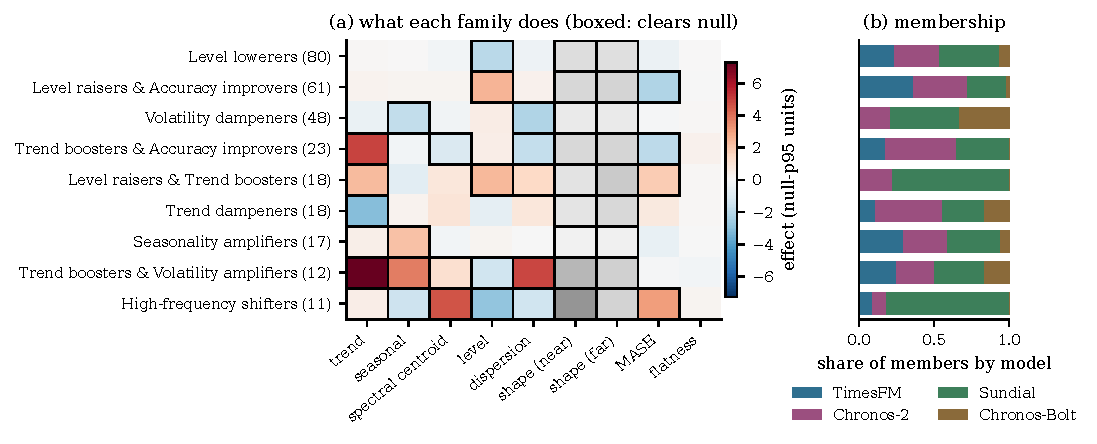
\includegraphics[width=\textwidth]{families.pdf}
\caption{The nine causal-effect families. (a) Family centroid in null units, signed as what the feature does
(red raises, blue lowers; boxed cells clear the null; shape distances unsigned, gray). (b) Membership by model. Source: \texttt{sae/concept\_families.json}.}
\label{fig:families}
\end{figure}

\section{Finding 2: Each Model Implements the Response Its Own Way}
\label{sec:mechanisms}

Shared inputs and shared broad effects leave open whether the models share the \emph{mechanism}: the same
concept, with the same effect, on the same series. At that grain they do not.

\subsection{Fine-grained concepts are organized by model}
\label{sec:bymodel}

The atlas groups causal features from all models whose effect profiles agree at cosine 0.9. It finds more structure than
a column-shuffle null (11 concepts, null 95th percentile 5.05; $p=0.005$), but of the 11 concepts, none spans more than 3
of the 7 models. The clusters are purer by model than random assignment makes them: 9 multi-model concepts against a
null mean of 10.8 ($p_{\text{below}}=0.025$), mean model purity 0.591 against 0.474 (\fid{SH-22}). Five of the 11 are
\emph{convergent}: two models reach the same effect from different series. The result holds held-out: no concept of the
private atlas spans more than 3 of 7 models on v2 or more than 2 on v3 (\fid{SH-16}). Each architecture builds its own
variants of a level or seasonality effect, and several reach the same effect independently.

The clearest component-level example is seasonality. Restoring a deseasonalized context requires one attention head in
TimesFM, but a minimal set of five heads in Chronos-T5-Base whose contributions do not add (path-patching gap 0.0238
against a mean effect of 0.0108; \fid{CA-03}, exploratory). The same capability is a single component in one model and
a nonlinear circuit in another.

\subsection{The same effect on the same series is found only within the Chronos family}
\label{sec:sameeffect}

The strictest test ablates both sides of a reciprocal transfer on the same series. Of 1{,}290 tests, 216 are scorable
(Figure~\ref{fig:funnel}b): 7 show the same causal effect, 54 agree on level or shape alone, 133 show no specific
agreement and 22 act differently. All 7 ``same'' verdicts are between Chronos-2 and Chronos-Bolt, two models from one
family, six of them through one feature set in Chronos-Bolt's fourth block. Because the test never produces a false
``same'' on the planted forecaster, these detections stand. Its insensitivity means that their absence across families
does not prove that effects differ, and the 22 ``acts differently'' verdicts indicate that they sometimes do.
Correspondingly, no registered cross-model causal claim confirms held-out: three multi-model atlas concepts exceed the
null in centroid cosine on private data (0.955--0.988 against 95th percentiles 0.854--0.907) but fail the registered
member-pair rule, and 0 of 6 shared-input agreement claims confirm.

\begin{figure}[!tb]
\centering
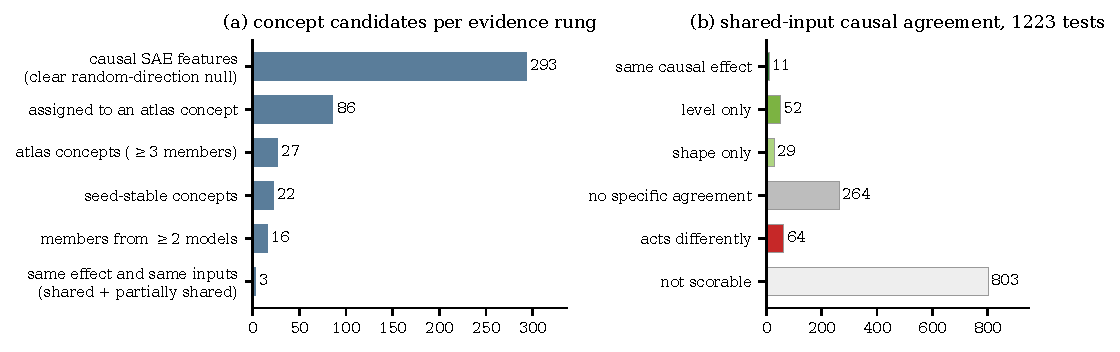
\includegraphics[width=\textwidth]{funnel.pdf}
\caption{(a) Concept candidates at each rung (the first three bars are sequential; the last three are properties of the
11 atlas concepts). (b) Same effect on the same inputs, over 1{,}290 tests drawn from the 1{,}296 reciprocal transfers:
only 7 are ``same'', all within the Chronos family. Source: \texttt{sae/concept\_stage.json}.}
\label{fig:funnel}
\end{figure}

\subsection{Forecast-relevant information is distributed}
\label{sec:distributed}

\paragraph{Causal features exist.} Of 56 target layers, 55 pass both reach controls. Across them, 442 feature-channel
cells clear the isotropic null where the empirical chance rate predicts 178.75 (2.47 times chance), from 1.64 times
(Chronos-T5-Base) to 5.70 (Chronos-Bolt). Timer is the exception: its layers reach the forecast, but its features clear
at 1.02 times chance (\fid{PM-17}). Target by target, 22 of 55 targets clear significantly more cells than chance, at
least two in every model except Timer. Registered single-feature effects replicate in part: 10 of 31 testable claims
confirm on the v2 private split, each at the Holm floor for 31 tests ($p_{\text{Holm}}=0.031$), and 11 of 24 on v3.

\paragraph{But single features are only weakly special.} The v3 run scored every feature against both nulls. Under the
isotropic null, 238 of 967 scorable features clear at least one channel; under the covariance-matched null, 91 do.
Scoring each null draw as a pseudo-feature on all nine channels at once gives expected counts of 67.0 and 70.4, so
features exceed chance 3.55-fold against isotropic directions ($p=4\times10^{-86}$) but only 1.29-fold against directions
drawn from the activation distribution ($p=0.0045$). Removing a typical on-manifold direction moves the forecast nearly
as much as removing a dictionary feature. The effects are also small: the median single-feature effect is 0.097 context
standard deviations, 2.2 times smaller than the 0.214 by which substituting the reconstruction moves the forecast (v3:
1.7 times; \fid{MN-15}).

\paragraph{Effects persist under other interventions, but the clearing set shifts.} We re-tested the 91 v3 features
that clear the on-manifold null under three on-manifold interventions, each with its own matched null: replacing the
feature by its corpus mean, by its activation on another series where it fires, or subtracting it from the model's own
activation rather than the reconstruction. 79 of 91 clear under at least one and 37 under all three; mean and resample
ablation keep the direction of the effect (median cosine to zero ablation 0.997 and 0.991; \fid{MP-10}). Most causal
features have a real effect, but which ones clear depends on the intervention.

\paragraph{Effects form a continuum, not discrete units.} Within a layer, 50 of 56 targets are non-modular: no
choice of $k$ splits their effect vectors into clusters of at least three members each. The families of
Section~\ref{sec:families} cover 192 of 194 features but do not beat a column-shuffle null in number ($p=0.68$), and the
silhouette is 0.25--0.32 for every cut from 6 to 16 families. The effect vectors are not low-dimensional (participation
ratio 5.58 of 9 channels on v3; \fid{MN-07}), so the absence of discrete units is not a lack of variation. Combined with
the on-manifold result, the picture is of forecast-relevant information spread across many directions, graded rather
than modular. This is a different picture from the monosemantic units sought in language models
\citep{bricken2023monosemanticity}, and it implies that a single-feature claim about a TSFM should be stated against an
on-manifold null.

\section{Finding 3: Shortcuts from Language-Model Interpretability Mislead}
\label{sec:shortcuts}

Several practices that are standard or natural when interpreting language models give wrong answers on TSFMs. Each
of the following was caught by a control and would otherwise have produced a confident, publishable result.

\paragraph{Averaging tokens hides shared geometry.} Section~\ref{sec:geometry} showed that the window average, the usual
way to compare models with different token widths, understates TimesFM's held-out similarity to four fine-token models
by 0.30--0.43 CKA. On mean-pooled representations, TimesFM/Chronos-2 is the 15th most similar of 21 pairs by CKA,
although it is the most similar pair by error agreement (0.948); with concatenated windows it rises to 9th on v2 and 7th
on v3. Conclusions about which TSFMs are alike therefore depend on a pooling choice that is usually not reported.

\paragraph{Activation prominence does not identify causal importance.} Ranking dictionary features by how strongly or
how often they fire, the default entry point of SAE analyses, selects mostly inert features: of the 927 most prominent
features of the v2 private atlas, 0.835 have no causal effect on the forecast (one-sided lower bound 0.817; dev 0.810;
$p_{\text{Holm}}=0.0005$; \fid{MN-14}), and on v3 the share is 0.919 of 861. Ranking by measured effect works: zeroing a
layer's five attribution-ranked atoms produces a median 0.74 share of the forecast change the dictionary can express,
more than activation-matched random sets of five atoms on 30 of 31 targets (\fid{D-42C}).

\paragraph{Attention mass is not causal importance.} The attention mass a head places on seasonal lags is uncorrelated
with the seasonal power lost when the head is ablated ($\rho=0.026$ in TimesFM and $-0.118$ in Chronos-T5-Base;
\fid{CA-04}), extending \citet{jain2019attention} to forecasting. Heads that look periodic are not the heads that carry
periodicity.

\paragraph{Correlation with a ground-truth factor is not control of it.} With exact generative ground truth, 154 of
10{,}240 TimesFM features and 115 of 6{,}144 Chronos-T5-Base features correlate with a generative field beyond a
permutation null, the strongest with intermittency ($\rho=0.881$; \fid{MP-06}). The correspondence is not specific:
moving the generator parameter along a dose ladder moves the matched feature no more than random features of matched
activation (0 of 151 registered tests survive correction; \fid{MN-17}). Steering the feature best matched to seasonal amplitude moves the forecast's seasonality in the
predicted direction in TimesFM and in the opposite direction in Chronos-T5-Base, in two independently trained
dictionaries each (\fid{CA-05}, exploratory). A feature that ``is'' seasonality by correlation can act against it.

\paragraph{The null decides the count.} Whether a feature is causal is decided against a random intervention, and the
choice of random intervention changes the answer severalfold. A null that removes a uniform,
batch-averaged amount rather than each token's own amount inflates the number of causal features 2.7-fold (110 to 293)
and fails the planted-forecaster test on every seed (Section~\ref{sec:knownanswer}). Between two nulls that both pass,
directions drawn isotropically and directions drawn from the activation distribution, the excess over chance falls from
3.55-fold to 1.29-fold (Section~\ref{sec:distributed}).

\paragraph{Similarity metrics do not agree on which models are alike.} Seven pairwise similarity metrics, from geometry
to error agreement to concept transfer, rank the 21 model pairs inconsistently (Kendall's $W=0.25$, $p=0.0095$;
\fid{SH-05}, \fid{SH-06}), and geometry does not track lineage: two untrained Chronos-T5 models are more similar (CKA 0.878) than the trained,
related Chronos-T5-Small and Base (0.734; \fid{MN-01}). A single ``model similarity'' number would hide these disagreements, so we report each metric against
its own null and never pool them.

\section{Depth and Practical Value}
\label{sec:depth}

\paragraph{Depth profiles.} For each of nine input corruptions, a model's sensitivity
fingerprint is the relative change of its residual stream at each layer; two models are compared by the rank
correlation of their fingerprints on a shared relative-depth axis; activations are never moved between models. For
TimesFM and Chronos-2 the agreement replicates on the v2 private split for 6 of 9 corruptions (overall $\rho=0.524$
[0.504, 0.544]; Figure~\ref{fig:heldout}a) and for 4 of 9 on v3, with 8 of 9 keeping their sign. The two models react at
matching depths to detrending (private $\rho=0.368$) and dropout (0.510), and at opposite depths to noise ($-0.743$),
spikes ($-0.785$) and warps ($-0.651$). Frequency shift (0.381 against 0.216 on dev) and smoothing ($-0.581$ against
$-0.418$) fail the registered rule because the agreement is stronger on private data than on dev. Only for level shift
is the agreement unstable; it changes sign between dev and private on both corpora (\fid{CA-01}).

\paragraph{Window-level restoration.} Patching clean activations window by window into a
corrupted TimesFM pass shows that the forecast is restored mainly in the window just before the horizon, increasingly so with
depth (from 0.427 of the damage undone at layer 0 to 0.612 at layer 8 and 0.631 at layer 16 for noise), while restoration
in the first window falls from $-0.191$ to 0.000 (320 series; \fid{DE-01}). This recency effect is
not visible when whole layers are patched.

\paragraph{Comparability of depth.} The captured blocks account for 13.9\%
(Chronos-T5-Base, encoder only) to 99.8\% (Timer) of a forecast's FLOPs (\fid{DE-05}), and on a whole-stack depth axis
Chronos-T5's last encoder block sits at depth 0.478 (\fid{DE-04}). Which layers appear most important also depends
strongly on the selection criterion (\fid{DE-08}). We therefore compare depth profiles across models rather than
the locations of single layers.

\paragraph{Failure prediction.} For each model we predict a series' log MASE from
free, output-only features (quantile width, forecast flatness, catch22 features of the context;
\citealp{lubba2019catch22}), add dictionary-family activations, and measure the gain, cross-fitted with a series
bootstrap. The free baseline is strong (Spearman 0.76--0.85), and for five models the gain's interval includes zero. The
gain is positive for the two least accurate models, Timer (+0.030 [0.019, 0.043]) and Time-MoE (+0.012 [0.005,
0.019]), and both confirm on the private split (Timer 0.0446 [0.0292, 0.0605], $p_{\text{Holm}}=0.002$; Time-MoE 0.011
[0.0032, 0.0194], $p_{\text{Holm}}=0.012$) and again on v3 (\fid{MN-28}). Internals do not help in choosing a model. Routing
each series to the model with the lowest predicted MASE gives 1.964 [1.837, 2.093] with internals against 1.948 [1.814,
2.070] without, both worse than always using Chronos-2 (1.856). For the more accurate models, the
model's output carries as much information about its errors as its internal features do.

\FloatBarrier
\section{Discussion}
\label{sec:discussion}

\paragraph{Convergence on inputs, not on mechanisms.} Seven forecasters with different tokenizers, depths and training
objectives single out the same series for a concept, share whole-layer geometry, and contain features with the same
broad effects: raising or lowering the forecast's level and damping or amplifying its seasonality. At the grain of
individual causal effects the convergence stops. Fine concepts are organized by model, the same capability can be one
head or a five-head circuit, and the same effect on the same series is detected only within one model family. One
reading consistent with all of this is that the models converge on \emph{what} in a series is predictive, which the
data dictate, while the \emph{implementation} of the response is left to each architecture. This is a weaker form of
convergence than the shared representations argued for in vision and language \citep{li2016convergent,huh2024platonic},
and our instruments locate where it stops: agreement on inputs is measurable and replicates, whereas agreement on effects
across architecture families is below what single-feature ablation resolves at these effect sizes.

\paragraph{What this means for interpreting TSFMs.} First, a single dictionary feature in a TSFM is only weakly special
against directions the model actually uses, so single-feature claims should be stated relative to an on-manifold null,
and the field's growing body of single-model SAE results
\citep{mishra2026dissecting,oublal2026timesae,divo2026zeitgeist} should be read with that in mind. Second, which
features matter must be measured by intervention: activation prominence, attention mass and correlation with a
generative factor each point at the wrong components. Third, cross-model comparison needs a measured time axis and a
pooling that keeps within-window order; otherwise similarity is understated by up to 0.43 CKA. Fourth, exploratory
pipelines with thousands of comparisons \citep{gelman2014garden} benefit from registration and a one-shot held-out test,
which here confirmed between half and two thirds of the registered claims (43 of 82 and 41 of 63) and sorted the
claim types cleanly into those that replicate and those that do not.

\section{Limitations}
\label{sec:limitations}

\paragraph{Models and alignment.} The study covers seven transformer models with contiguous tokens; models whose tokens
read disjoint lags, such as Lag-Llama, are out of scope. With seven models, differences between models are confounded
with architecture, size and training data, and Timer's features do not exceed chance, so its results carry no evidence
about causal concepts. The analysis is univariate (Chronos-2's cross-series attention is not measured; \fid{PM-13}), and
Chronos-T5's decoder and Sundial's flow head are not captured. The common time grid is no finer than the coarsest token,
and peak layer locations, unlike the size of similarity, depend on the window size (\fid{SH-23}). Dictionaries are
trained on window vectors, which is conservative for one-step models (\fid{MP-11}).

\paragraph{Ground truth and scope.} Ground truth is exact only for the synthetic tier and encodes the generators'
assumptions, and overlap with the models' pretraining data cannot be verified. Raw real benchmarks are a weaker basis for
causal questions, because weakly predictable real series receive flat forecasts in 67--100\% of cases (\fid{BM-06};
cf.\ \citealp{wan2026collapse}), leaving an ablation nothing to move; real data therefore enter as real-derived series
and as the external test set on which the transfer claims confirm. The confirmed transfers derive from two source
concepts on v2 and three source models on v3, so the shared-input result rests on few concepts. Concept results depend
on dictionary size, sparsity and seed; three replicate seeds measure this dependence but cannot remove it.

\section{Conclusion}
\label{sec:conclusion}

Across seven time-series foundation models and two independent corpora, with every causal instrument validated on a
planted known answer and every registered claim tested once on sealed data, architectures that look nothing alike agree
on what in a series matters---they share representational geometry, select the same inputs for a concept and contain
features that raise or lower the forecast's level and damp its seasonality---but implement the response in
model-specific, distributed ways. Several habits carried over from language-model interpretability, from averaging
tokens to trusting prominent features and attention maps, give confidently wrong answers on these models. The
benchmark, the analysis system and every result with its reproduction command are public, so each conclusion can be
re-tested on new models as they appear.

\paragraph{Availability.} Code (MIT license), configurations, the example run and the findings ledger are at
\url{\repourl}. Version 1.1.0 is archived at \href{https://doi.org/10.5281/zenodo.23267462}{doi:10.5281/zenodo.23267462},
and both packages install from PyPI (\texttt{pip install tsfm-lens tsfm-benchmark}).


\acks{Computational resources were provided by the second author's lab at Rutgers University. This work received no
external funding, and the authors declare no competing interests. Use of AI tools: Claude (Anthropic) wrote most of the
repository's code and tests, ran the experiments and helped draft and edit the manuscript, under the authors' direction.
The research questions, ideas and general design choices are the authors', who reviewed the implementation details Claude
proposed, checked every reported result and take full responsibility for the content.}

\appendix
\section{The Analysis System}
\label{app:system}

All analyses are produced by \tool{}, which consists of two separately installable packages. \texttt{tsfm\_benchmark}
generates, leakage-audits, seals and validates corpora; \texttt{tsfm\_lens} loads checkpoints through adapters, runs a
gated pipeline of 19 analysis stages and renders one self-contained HTML report (Figure~\ref{fig:overview}). A zero-code
adapter for Hugging Face checkpoints discovers layers and measures token spans, and loads two of the seven models here
(Timer and Time-MoE). Stages a model cannot support are skipped with a reason rendered in the report; every intervention
goes through one patching primitive, which raises if the model silently splits a batch; and the \texttt{confirm} stage
refuses mismatched registry hashes, requires the private seal to verify and refuses to overwrite its own artifact. The
system and its design are described in a companion software paper; usage is documented in the repository.

\begin{figure}[!tb]
\centering
% System architecture figure, shared by ../main.tex (Figure 1) and ../mloss/main.tex.
% Needs the colors `accent` and `soft` and the TikZ libraries positioning, fit, backgrounds.
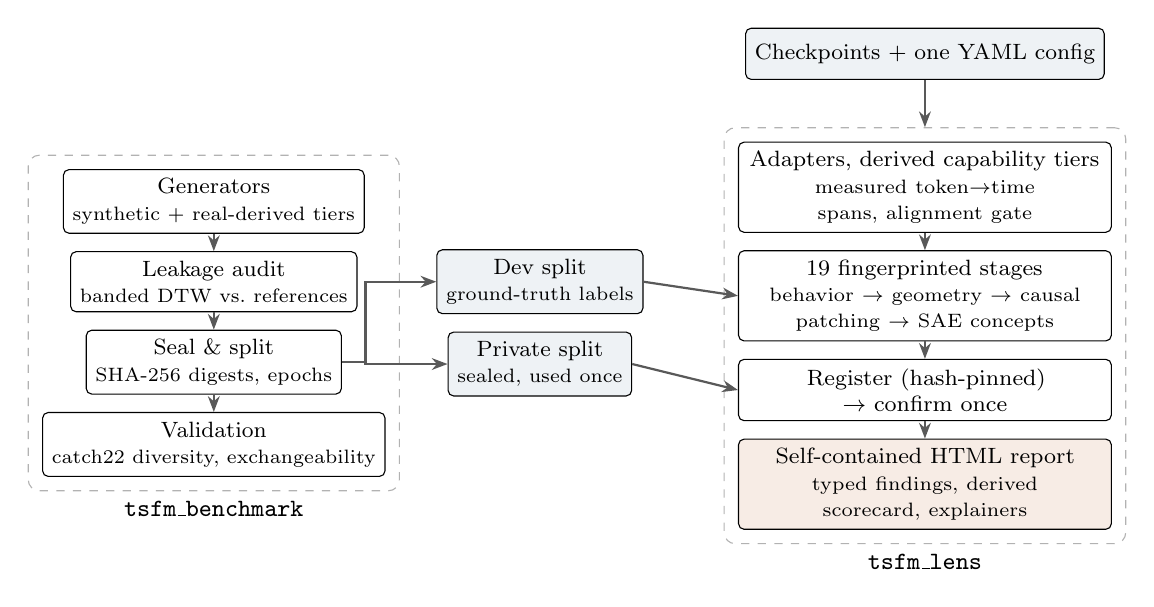
\begin{tikzpicture}[
  node distance=2.2mm and 6mm,
  box/.style={draw, rounded corners=2pt, align=center, font=\footnotesize, minimum height=6.5mm, fill=white},
  pkg/.style={draw=gray!60, dashed, rounded corners=4pt, inner sep=5pt},
  arr/.style={-{Stealth[length=2mm]}, thick, gray!70!black}]
  \node[box] (gen) {Generators\\{\scriptsize synthetic + real-derived tiers}};
  \node[box, below=of gen] (aud) {Leakage audit\\{\scriptsize banded DTW vs.\ references}};
  \node[box, below=of aud] (seal) {Seal \& split\\{\scriptsize SHA-256 digests, epochs}};
  \node[box, below=of seal] (val) {Validation\\{\scriptsize catch22 diversity, exchangeability}};
  \draw[arr] (gen) -- (aud); \draw[arr] (aud) -- (seal); \draw[arr] (seal) -- (val);
  \begin{scope}[on background layer]
    \node[pkg, fit=(gen)(val), label={[font=\small\bfseries]below:\texttt{tsfm\_benchmark}}] {};
  \end{scope}
  \node[box, right=10mm of aud, fill=soft] (dev) {Dev split\\{\scriptsize ground-truth labels}};
  \node[box, below=of dev, fill=soft] (priv) {Private split\\{\scriptsize sealed, used once}};
  \draw[arr] (seal.east) -- ++(3mm,0) |- (dev.west);
  \draw[arr] (seal.east) -- ++(3mm,0) |- (priv.west);
  \node[box, right=12mm of dev, yshift=12mm, text width=45mm] (ad) {Adapters, derived capability tiers\\{\scriptsize measured token$\to$time spans, alignment gate}};
  \node[box, below=of ad, text width=45mm] (st) {19 fingerprinted stages\\{\scriptsize behavior $\to$ geometry $\to$ causal patching $\to$ SAE concepts}};
  \node[box, below=of st, text width=45mm] (reg) {Register (hash-pinned) $\to$ confirm once};
  \node[box, below=of reg, text width=45mm, fill=accent!12] (rep) {Self-contained HTML report\\{\scriptsize typed findings, derived scorecard, explainers}};
  \draw[arr] (ad) -- (st); \draw[arr] (st) -- (reg); \draw[arr] (reg) -- (rep);
  \begin{scope}[on background layer]
    \node[pkg, fit=(ad)(rep), label={[font=\small\bfseries]below:\texttt{tsfm\_lens}}] (lens) {};
  \end{scope}
  \draw[arr] (dev.east) -- (st.west);
  \draw[arr] (priv.east) -- (reg.west);
  \node[box, above=6mm of lens.north, fill=soft] (ck) {Checkpoints + one YAML config};
  \draw[arr] (ck) -- (lens.north);
\end{tikzpicture}

\caption{System overview. \texttt{tsfm\_benchmark} produces leakage-audited, sealed corpora with exact ground truth;
\texttt{tsfm\_lens} turns a configuration naming checkpoints into one report. Dev findings are exploratory; the private
split is opened once, by \texttt{confirm}, for claims registered in advance.}
\label{fig:overview}
\end{figure}

\section{Model Behavior}
\label{app:behavior}

\begin{table}[!tb]
\centering
\footnotesize
\setlength{\tabcolsep}{4pt}
\begin{tabular}{@{}lccccc@{}}
\toprule
Model & median MASE & 80\% coverage & scale resid.\ (s.d.) & missing value & latency (ms) \\
\midrule
\textcolor{ctwo}{Chronos-2}    & \textbf{1.2002} & 0.757 & 0.0102 & handled & 23 \\
\textcolor{tfm}{TimesFM}       & 1.2560 & \textbf{0.779} & $1.6\times10^{-6}$ & propagates & 39 \\
\textcolor{sun}{Sundial}       & 1.4131 & 0.360 & 0.0310 & propagates & 62 \\
\textcolor{tt5}{Chronos-T5-Base} & 1.4231 & 0.436 & $2.7\times10^{-7}$ & handled & 975 \\
\textcolor{bolt}{Chronos-Bolt} & 1.5487 & 0.732 & 0.0101 & handled & 15 \\
\textcolor{timer}{Timer}       & 1.9306 & -- & 0.0262 & propagates & 5 \\
\textcolor{tmoe}{Time-MoE}     & 2.8642 & -- & 0.0368 & propagates & 103 \\
\midrule
naive / seasonal naive & 2.7593 / 1.9819 & & & & \\
\bottomrule
\end{tabular}
\caption{Behavior on the v2 dev split (965 series). Scale residual: error of $f(c\,x)/c$ against $f(x)$ in context
standard deviations, $c=0.001$. Missing value: whether an injected NaN is handled or propagates silently. Latency: median
time to forecast a batch of 8 series. Timer and Time-MoE output point forecasts only.}
\label{tab:character}
\end{table}

Table~\ref{tab:character} summarizes behavior on the v2 dev split. Five models beat the seasonal-naive forecast on
76.5--84.5\% of series, Timer on 69.5\% and Time-MoE on only 37.8\%. The nominal 80\% intervals of Sundial and
Chronos-T5-Base cover only 36\% and 44\% of outcomes, and four models propagate an injected missing value silently. On
the private split, Chronos-2 is more accurate than TimesFM overall, with a smaller effect than on \texttt{mixture}
($-0.070$ [$-0.129$, $-0.008$], $p=0.025$, $n=971$). Sampled models (Sundial, Chronos-T5) are seeded identically in every
compared pair of calls: unseeded, back-to-back Sundial calls differ by up to 0.50 MASE (\fid{PM-09}).

\section{Statistical Details and Validity}
\label{app:stats}

\paragraph{Paired series bootstrap.} With per-series differences $d_s=m_{a,s}-m_{b,s}$ and $B=n_{\text{boot}}=5000$
resampled means $\bar d^*_b$, the interval is the percentile interval and
$p=\min\!\big(1,\max(\tfrac1B,\,2\min\{\tfrac1B\#(\bar d^*_b\le 0),\tfrac1B\#(\bar d^*_b\ge 0)\})\big)$
\citep{phipson2010permutation}. Window-level statistics (CKA, fingerprints) resample series with all their windows
\citep{cameron2008cluster}.

\paragraph{Multiplicity.} Confirmatory families use Holm, $\tilde p_{(i)}=\max_{j\le i}\min(1,(m-j+1)p_{(j)})$
\citep{holm1979}; with $p\ge 1/B$ the smallest attainable value is $m/B$, which is checked per family. Atlas transfer
uses Benjamini--Hochberg \citep{benjamini1995fdr}. The v2 run has 123 test families with 4{,}238 comparisons; the
8{,}705 feature-channel cells of the ablation battery are judged by their count against the empirical chance rate,
which ranged from 0.3\% to 4\% per target.

\paragraph{Ablation nulls.} For feature $i$ with rows $R_i$ and $J=16$ unit directions $u_j$, the null removes at every
token $t$ the amount $|z_i(t)|\,\|w_i\|\,u_j$. In the isotropic null $u_j$ is $W_d^{\top}r_j$ normalized, with $r_j$ a
random unit code; in the covariance-matched null $u_j\propto\sum_t g_{jt}(x_t-\bar x)$ with $g_{jt}\sim\mathcal{N}(0,1)$
over the chunk's clean token activations $x_t$. Channel $c$ clears if
$\frac{1}{|R_i|}\sum_{r\in R_i}|\Delta^{(c)}_{i,r}| > q_{0.95}\{|\Delta^{(c)}_{u_j,r}|: j\le J, r\in R_i\}$.

\paragraph{Transfer.} The statistic is $\max_f \mathrm{AUC}(a_f;S)$ over destination features; its null recomputes the
same maximum on stratum-matched random $k$-sets, so the feature search is inside the null. A registered claim uses
$\max(p,p_{\text{rev}})$ over the two directions, Holm across claims.

\paragraph{Power.} Before the private result is read, each claim's minimum detectable effect is simulated by shifting
recentred per-series differences and re-testing with the same bootstrap (for example $\Delta$MASE 0.133 at $n=290$, 80\%
power, against an observed 0.209). The 20 transfer claims all reach the Holm floor. Single-feature causal claims are
power-limited: each feature is tested on its 8 strongest-firing series, and 19 of the 21 v2 claims that did not confirm
had not reached the dev $p$ floor.

\paragraph{Benchmark and dictionaries.} Every v2 sample passed the banded-DTW leakage gate (threshold 0.35; closest
accepted sample 0.352), and 6 of 937{,}015 dev--private pairs are near-duplicates. Each target has three replicate
dictionaries, and 9 of 11 atlas concepts are stable across them; held-out fraction of variance explained has medians of
0.647 (TimesFM) to 0.878 (Chronos-T5-Base), and fidelity does not predict causal clarity across v3 targets ($\rho=-0.326$,
$n=49$; \fid{MN-34}). Retraining the v3 dictionaries from the recorded configuration reproduced all 50 exactly and the
same 91 causal features.

\paragraph{Integrity of the confirmation.} The v2 registry (128 hypotheses, sha256 recorded) was frozen before the
private epoch was generated; the epoch shares no sample hash with any of seven earlier splits, and \texttt{confirm} ran
once. Registered claims are cuts from larger dev pools (transfer 20 of 1{,}124 candidates, causal 32 of 113), which is
legitimate because the private split referees them. The v3 registry (111 hypotheses) and the window-geometry claims were
frozen in the same way before their epochs were extracted.

\section{Reproducibility}
\label{app:repro}

\repodir{examples/panel7_v2} holds the configuration, the report and every stage's JSON and parquet artifacts plus the
confirmation; \texttt{paper/figures/make\_figures.py} regenerates all data figures. From \texttt{tsfm\_lens/},
\texttt{python run.py -{}-config configs/panel7\_v2.yaml} reproduces the run. Environment: Python 3.12.13, numpy 2.1.0,
PyTorch 2.12.0 (CUDA 12.9), transformers 4.57.6, timesfm 2.0.2, chronos-forecasting 2.3.1, zarr 2.18.7, scikit-learn
1.7.2. The v2 run took 21.1 hours on one RTX A5000.


{\footnotesize\setlength{\bibsep}{0pt}\bibliography{../references}}

\end{document}
